% ══════════════════════════════════════════════════════════════════════════════
%  Digital Twin-Driven Flood Evacuation System Augmented with Agentic AI
%  via Model Context Protocol
%  ──────────────────────────────────────────────────────────────────────────
%  IEEE Journal Format  |  ~10 pages  |  2026
% ══════════════════════════════════════════════════════════════════════════════

\documentclass[journal]{IEEEtran}

% ── Packages ──────────────────────────────────────────────────────────────────
\usepackage{cite}
\usepackage{amsmath,amssymb,amsfonts}
\usepackage{graphicx}
\usepackage{textcomp}
\usepackage{xcolor}
\usepackage{booktabs}
\usepackage{multirow}
\usepackage{hyperref}
\usepackage{tabularx}
\usepackage{array}
\usepackage{listings}
\usepackage{url}
\usepackage{balance}
\usepackage{float}
\usepackage{enumitem}
\usepackage{subcaption}

% ── Code listing style ────────────────────────────────────────────────────────
\definecolor{codegreen}{rgb}{0.0,0.5,0.0}
\definecolor{codegray}{rgb}{0.5,0.5,0.5}
\definecolor{codepurple}{rgb}{0.58,0,0.82}
\definecolor{backcolour}{rgb}{0.96,0.96,0.96}

\lstdefinestyle{mcpstyle}{
    backgroundcolor=\color{backcolour},
    commentstyle=\color{codegreen},
    keywordstyle=\color{codepurple},
    numberstyle=\tiny\color{codegray},
    stringstyle=\color{red!60!black},
    basicstyle=\ttfamily\scriptsize,
    breaklines=true,
    frame=single,
    captionpos=b,
}
\lstset{style=mcpstyle}

% ── Hyperref setup ────────────────────────────────────────────────────────────
\hypersetup{
    colorlinks=true,
    linkcolor=blue!60!black,
    citecolor=blue!60!black,
    urlcolor=blue!60!black,
}

% ══════════════════════════════════════════════════════════════════════════════
\begin{document}

\title{Digital Twin-Driven Flood Evacuation System Augmented with Agentic AI via Model Context Protocol}

% TODO: Replace with actual author names and affiliations
\author{
    Author~One,~Author~Two,~and~Author~Three%
    \thanks{Authors are with the Department of Computer Science and Engineering,
    University Name, Bangalore, India.
    E-mail: \{author1, author2, author3\}@university.edu}
}

\markboth{IEEE Journal, Vol.~XX, No.~XX, Month~2026}%
{Author \MakeLowercase{\textit{et al.}}: Digital Twin-Driven Flood Evacuation with MCP-Based Agentic AI}

\maketitle

% ══════════════════════════════════════════════════════════════════════════════
%  ABSTRACT
% ══════════════════════════════════════════════════════════════════════════════
\begin{abstract}
Urban flooding events present complex, multi-domain challenges that demand
intelligent, context-aware evacuation systems capable of reasoning across
simulation data, infrastructure status, transportation networks, and resource
logistics simultaneously. This paper presents a novel system that combines
Digital Twin technology with Agentic AI powered by the Model Context Protocol
(MCP) for urban flood evacuation management. Unlike traditional approaches
that rely on static evacuation plans or monolithic retrieval-augmented
generation (RAG) pipelines, our architecture deploys six specialized MCP
servers exposing 28 tools that enable autonomous AI agents to selectively
query, reason over, and act upon Digital Twin simulation state across distinct
operational domains. We introduce a Context Tree pipeline that transforms raw
simulation output---including physics-based flood modeling via Manning's
equation and the Height Above Nearest Drainage (HAND) model---into enriched,
tool-level selective context, eliminating the token overflow problem inherent
in full-context retrieval approaches. Evaluated through a case study in
Bangalore, India, our system demonstrates that MCP-based agentic architectures
achieve 77.5\% average reduction in context token consumption compared to
traditional RAG (exact measurements via Gemini API token counter, across five disaster response queries), while enabling
multi-domain autonomous reasoning across evacuation operations, flood intelligence,
and transportation logistics that is fundamentally impossible with single-index
retrieval or direct API integration patterns.
\end{abstract}

\begin{IEEEkeywords}
Digital Twin, Model Context Protocol, Agentic AI, Flood Evacuation,
Large Language Models, Urban Disaster Management, Multi-Agent Systems
\end{IEEEkeywords}

% ══════════════════════════════════════════════════════════════════════════════
%  I. INTRODUCTION
% ══════════════════════════════════════════════════════════════════════════════
\section{Introduction}
\label{sec:introduction}

\IEEEPARstart{U}{rban} flooding has emerged as one of the most consequential
natural hazards of the 21st century, amplified by rapid urbanization, climate
change, and aging drainage infrastructure. Cities in tropical and monsoon
regions are disproportionately affected: Bangalore, India, received over
800\,mm of rainfall during the 2022 monsoon season, displacing more than
25,000 residents and causing an estimated \$225 million in damages~\cite{ndma2022}.
Traditional flood evacuation systems rely on pre-computed static plans that
fail to account for the dynamic, multi-modal nature of urban flood events---
where road passability, shelter capacity, public transit availability, and
resource logistics change continuously as floodwaters advance.

Recent advances in Digital Twin technology offer a promising paradigm for
modeling and managing such complex urban systems. A Digital Twin provides a
synchronized digital replica of the physical environment, enabling simulation,
analysis, and what-if exploration in a virtual space~\cite{grieves2014digital,
tao2019digital}. When applied to flood management, Digital Twins can
integrate geospatial data, hydrological models, infrastructure networks, and
population distributions to create a living model of the crisis as it unfolds.

However, a critical gap persists between the data richness of Digital Twins
and the actionability of their outputs. Current systems either present raw
simulation data through dashboards---requiring human experts to manually
interpret and act---or employ simplistic AI integration through
Retrieval-Augmented Generation (RAG) pipelines that dump the entire simulation
context into a language model, leading to token overflow, hallucination, and
loss of domain-specific reasoning~\cite{lewis2020rag}.

This paper addresses this gap by introducing the \textbf{Model Context
Protocol (MCP)}~\cite{anthropic2024mcp} as the interface layer between a
physics-informed Digital Twin and autonomous AI agents. MCP, originally
proposed by Anthropic in 2024, provides a standardized protocol through which
AI models can discover, invoke, and compose tools exposed by external
servers---analogous to how USB-C provides a universal connector for
peripherals. By decomposing the Digital Twin's capabilities into domain-specific
MCP servers, each exposing focused, tool-level interfaces, we enable AI agents
to perform \emph{selective context retrieval}---querying only the specific
data slices relevant to the current reasoning step, rather than ingesting the
entire simulation state.

\subsection{Contributions}
The principal contributions of this work are:

\begin{enumerate}[leftmargin=*]
    \item \textbf{First MCP-based Agentic AI Architecture for Disaster
    Management:} We design and implement a multi-server MCP ecosystem
    comprising six specialized servers exposing 23+ tools for autonomous
    disaster response AI agents, demonstrating the protocol's applicability
    beyond its original software development domain.

    \item \textbf{Context Tree Architecture:} We introduce a structured
    pipeline that transforms raw Digital Twin simulation output into enriched,
    semantically organized context, enabling tool-level selective retrieval
    that reduces token consumption by up to 75\% compared to full-context
    RAG approaches.

    \item \textbf{Physics-Informed Digital Twin for Flood Simulation:} We
    develop a simulation engine that integrates Manning's equation hydraulics,
    the HAND model, SRTM digital elevation data, and live traffic feeds to
    produce physically grounded flood impact assessments over real urban road
    networks.

    \item \textbf{Comprehensive Evaluation of MCP vs.\ Traditional
    Architectures:} We provide a detailed comparative analysis of MCP-based
    selective context against RAG and direct API integration patterns,
    demonstrating MCP's superiority for large-context, multi-domain disaster
    response scenarios.
\end{enumerate}

The remainder of this paper is organized as follows. Section~\ref{sec:related}
reviews related work. Section~\ref{sec:architecture} presents the system
architecture. Section~\ref{sec:digitaltwin} describes the Digital Twin
simulation engine. Section~\ref{sec:mcp} details the MCP-based Agentic AI
architecture---the core contribution. Section~\ref{sec:comparison} provides
an expanded comparison of MCP against traditional approaches.
Section~\ref{sec:casestudy} presents a case study.
Section~\ref{sec:discussion} discusses findings and limitations, and
Section~\ref{sec:conclusion} concludes.


% ══════════════════════════════════════════════════════════════════════════════
%  II. RELATED WORK
% ══════════════════════════════════════════════════════════════════════════════
\section{Related Work}
\label{sec:related}

\subsection{Digital Twins for Disaster Management}
The concept of Digital Twins, introduced by Grieves~\cite{grieves2014digital}
and formalized by Tao et al.~\cite{tao2019digital}, has gained traction in
urban management. Ford and Wolf~\cite{ford2016smart} proposed Digital Twin
cities for infrastructure monitoring, while recent work has extended the
paradigm to disaster response. Existing Digital Twin systems for floods
typically focus on hydrological simulation~\cite{wing2017flood} or structural
monitoring, but lack the intelligent agent interface necessary for autonomous
decision support.

\subsection{AI and LLMs for Emergency Response}
Large Language Models (LLMs) have been explored for disaster situational
awareness~\cite{google2024gemini}, including document summarization,
damage assessment from social media, and resource allocation planning.
However, most implementations follow a passive RAG pattern where documents
are retrieved and concatenated into a prompt---a paradigm ill-suited for
the structured, multi-domain data produced by Digital Twin
simulations~\cite{lewis2020rag}.

\subsection{Model Context Protocol}
MCP, introduced by Anthropic in November 2024~\cite{anthropic2024mcp},
defines a client-server architecture where AI models act as MCP clients
that discover and invoke tools exposed by MCP servers via standardized
JSON-RPC messaging. While MCP has seen rapid adoption in software
development tooling (IDE integration, code analysis, database querying),
its application to disaster management remains unexplored. Our work
represents the first deployment of MCP in a safety-critical, multi-domain
operational context.

\subsection{Tool-Using AI Agents}
The ReAct paradigm~\cite{yao2023react} demonstrated that LLMs can
interleave reasoning and action through tool invocation. Function calling
capabilities in modern LLMs (Gemini, GPT-4, Claude) have formalized this
into structured tool-use interfaces. Our system leverages this capability
within the MCP framework, where each MCP server provides a semantically
rich tool catalog that the AI agent can autonomously navigate.

\subsection{Metaheuristic Optimization for Evacuation}
Genetic Algorithms~\cite{holland1975adaptation, goldberg1989ga}, Particle
Swarm Optimization~\cite{kennedy1995pso}, and Ant Colony
Optimization~\cite{dorigo2004aco} have been extensively studied for
evacuation route planning. Our system employs all three algorithms within
a fair comparison framework, though this paper focuses on the MCP-based
AI architecture rather than algorithmic comparison, which is the subject of
a companion study.


% ══════════════════════════════════════════════════════════════════════════════
%  III. SYSTEM ARCHITECTURE
% ══════════════════════════════════════════════════════════════════════════════
\section{System Architecture}
\label{sec:architecture}

The proposed system follows a five-layer architecture, depicted in
Fig.~\ref{fig:architecture}, designed to separate concerns between
simulation, optimization, AI reasoning, data persistence, and user
interaction.

% ── FIGURE 1: System Architecture ─────────────────────────────────────────────
\begin{figure*}[!t]
    \centering
    \includegraphics[width=0.95\textwidth]{figures/system_architecture.png}
    \caption{System architecture of the proposed Digital Twin-driven flood
    evacuation system with MCP-based Agentic AI. The five layers---
    presentation, application, simulation, intelligence, and data---communicate
    through well-defined interfaces, with the MCP layer serving as the bridge
    between the Digital Twin's structured state and autonomous AI reasoning.}
    \label{fig:architecture}
\end{figure*}

\textbf{Layer 1 --- Presentation (React Frontend):} A web-based interface
built with React and Vite, featuring 30 components including interactive
flood maps (Leaflet), evacuation route visualization, AI expert panels with
streaming responses, and a conversational copilot. Key components include
\texttt{FloodMap.jsx} for geospatial visualization, \texttt{PanelOfExperts.jsx}
for AI expert streaming, and \texttt{AppCopilot.jsx} for agentic conversation.

\textbf{Layer 2 --- Application (FastAPI Backend):} A Python FastAPI server
(\texttt{service.py}, 1599 lines) orchestrating the simulation pipeline:
region loading via OSMnx, flood computation, shelter discovery through
OpenStreetMap Overpass API, population overlay from census data, and
optimization algorithm execution. Results are streamed to the frontend via
Server-Sent Events (SSE).

\textbf{Layer 3 --- Simulation (Digital Twin Engine):} The physics-informed
flood simulation core, detailed in Section~\ref{sec:digitaltwin}, combining
Manning's equation, the HAND model, and SRTM DEM elevation data to produce
physically grounded flood depth estimates across the urban road network.

\textbf{Layer 4 --- Intelligence (MCP Server Hub):} Six specialized MCP
servers, detailed in Section~\ref{sec:mcp}, that expose the Digital Twin's
state as composable tools for autonomous AI reasoning. This layer also
includes the Context Tree pipeline (\texttt{context\_builder.py}), expert
persona system, and multi-model reliability layer.

\textbf{Layer 5 --- Data (MongoDB + External APIs):} A MongoDB database with
15+ collections storing population data, resource inventories (IDRN, fire
stations, SAR equipment), metro network topology, region graph caches, and
simulation state. Eleven external APIs provide live data feeds (Table~\ref{tab:apis}).

% ── TABLE I: MCP Server Ecosystem ─────────────────────────────────────────────
\begin{table*}[!t]
    \centering
    \caption{MCP Server Ecosystem: Six Specialized Servers Spanning Five Operational Domains}
    \label{tab:mcp_servers}
    \begin{tabular}{@{}llcl@{}}
        \toprule
        \textbf{MCP Server} & \textbf{Domain} & \textbf{Tools} & \textbf{Key Capabilities} \\
        \midrule
        Evacuation Operations & Simulation \& Ops & 12 &
            Simulation state, shelter status, route analysis, terrain, \\
        & & & strategy generation, rescue guidelines, weather, bus/transit \\
        \midrule
        Flood Intelligence & Strategic Analysis & 4 &
            Metro line-level health aggregation (CRITICAL/DEGRADED/ \\
        & & & OPERATIONAL), socio-economic impact, Super-Hub resource \\
        & & & mapping, vulnerability hotspot identification \\
        \midrule
        Transport GTFS & Logistics & 3 &
            BMTC bus stop proximity, route lookup, transit disruption \\
        & & & analysis using GTFS static feeds \\
        \midrule
        GIS Spatial & Geospatial & 3 &
            DEM ingestion, vector feature extraction, spatial clipping \\
        \midrule
        Weather & Environmental & 1 &
            Multi-source precipitation cascade (4-tier fallback) \\
        \midrule
        App Copilot & Frontend Control & 5 &
            Region selection, map navigation, simulation launch, \\
        & & & algorithm configuration, UI state management \\
        \midrule
        \multicolumn{2}{l}{\textbf{Total}} & \textbf{28} & \\
        \bottomrule
    \end{tabular}
\end{table*}


% ══════════════════════════════════════════════════════════════════════════════
%  IV. DIGITAL TWIN SIMULATION ENGINE
% ══════════════════════════════════════════════════════════════════════════════
\section{Digital Twin Simulation Engine}
\label{sec:digitaltwin}

The Digital Twin at the core of our system constructs a physics-informed model
of urban flood dynamics over real geospatial infrastructure, integrating five
data sources into a unified simulation environment.

\subsection{Urban Road Network Construction}
The road network graph $G = (V, E)$ is constructed using
OSMnx~\cite{boeing2017osmnx}, where nodes $V$ represent intersections and
edges $E$ represent road segments extracted from OpenStreetMap. Each node $v_i$
is annotated with geographic coordinates $(\text{lat}_i, \text{lon}_i)$ and
elevation $h_i$ obtained from the Shuttle Radar Topography Mission (SRTM)
30-meter Digital Elevation Model~\cite{farr2007srtm} via the OpenTopography
API. This elevation data enables terrain-aware routing---a critical requirement
for flood evacuation, where directing evacuees downhill toward pooling water
must be actively penalized.

\subsection{Flood Depth Estimation}
Flood depth at each node is computed using a two-model approach:

\textbf{Manning's Equation} provides the flow velocity through each road
segment, treating streets as open channels:
\begin{equation}
    v = \frac{1}{n} R^{2/3} S^{1/2}
    \label{eq:manning}
\end{equation}
where $v$ is flow velocity (m/s), $n$ is Manning's roughness coefficient
(calibrated per road surface type), $R$ is the hydraulic radius, and $S$ is
the energy slope derived from the elevation gradient between adjacent
nodes~\cite{manning1891, chow1959}.

\textbf{HAND Model.} The Height Above Nearest Drainage (HAND)
model~\cite{nobre2011hand, renno2008hand} estimates flood susceptibility by
computing the vertical distance from each node to the nearest drainage
channel. Nodes with low HAND values (i.e., close to drainage level) are
assigned higher flood depths for a given rainfall intensity:
\begin{equation}
    d_i = f(\text{rainfall}, \text{HAND}_i, h_i)
    \label{eq:flood_depth}
\end{equation}

The computed flood depths directly affect edge traversability through a
flood-weighted cost function:
\begin{equation}
    w_{\text{flood}}(e_{ij}) = \ell_{ij} \times (1 + 5.0 \times \bar{d}_{ij})
    \times \tau_{ij}
    \label{eq:flood_weight}
\end{equation}
where $\ell_{ij}$ is the road segment length, $\bar{d}_{ij}$ is the average
water depth across edge $e_{ij}$, and $\tau_{ij}$ is a traffic congestion
factor obtained from TomTom live traffic data when available.

\subsection{Shelter Discovery and Capacity Estimation}
Safe shelters are automatically discovered using the OpenStreetMap Overpass
API, querying for schools, hospitals, community halls, and designated relief
centers within the simulation region. Each shelter $s_j$ is characterized by
its capacity $C_j$ (estimated from building footprint area), geographic
coordinates, and a safety assessment based on local flood depth and elevation.
A shelter is marked unsafe if the surrounding flood depth exceeds a critical
threshold.

\subsection{Infrastructure Integration}
The Digital Twin additionally integrates:
\begin{itemize}[leftmargin=*]
    \item \textbf{Metro rail network:} Namma Metro (BMRCL) station
    coordinates, line topology, and per-station flood risk scores based on
    entrance elevation relative to surrounding road flood depths.
    \item \textbf{Public bus transit:} BMTC bus stop locations and route
    data from GTFS static feeds, enabling the AI agent to assess alternative
    evacuation transport.
    \item \textbf{Population distribution:} Census ward-level population
    densities overlaid onto the road network to estimate at-risk populations
    per node.
    \item \textbf{Weather data:} A four-tier weather cascade
    (WeatherAPI.com $\to$ MET Norway + wttr.in $\to$ wttr.in $\to$
    Open-Meteo) ensures precipitation data availability even under partial
    internet connectivity.
\end{itemize}

% ── FIGURE 3: Digital Twin Visualization ──────────────────────────────────────
\begin{figure}[!t]
    \centering
    \includegraphics[width=0.95\columnwidth]{figures/digital_twin_ui.png}
    \caption{Digital Twin visualization interface showing flood depth overlay
    (red = severe, yellow = moderate), computed evacuation routes (blue lines),
    and shelter markers with capacity indicators for a simulated 120\,mm
    rainfall event in Bangalore.}
    \label{fig:digital_twin}
\end{figure}


% ══════════════════════════════════════════════════════════════════════════════
%  V. MCP-BASED AGENTIC AI ARCHITECTURE
% ══════════════════════════════════════════════════════════════════════════════
\section{MCP-Based Agentic AI Architecture}
\label{sec:mcp}

The Model Context Protocol layer is the principal contribution of this work.
It transforms the Digital Twin from a passive data source into an active
intelligence platform by exposing simulation capabilities as composable tools
that autonomous AI agents can discover, invoke, and chain together to perform
complex, multi-step reasoning.

\subsection{Design Philosophy: Why MCP for Disaster AI}

Traditional approaches to integrating AI with simulation systems follow one
of two patterns:

\begin{enumerate}[leftmargin=*]
    \item \textbf{Full-context RAG:} The entire simulation state (shelter
    reports, route details, flood depths, resource inventories) is serialized
    and injected into the LLM prompt. For a typical Bangalore simulation with
    15 shelters, 200+ routes, and 338 resource items, this produces
    8,000--12,000 tokens of context per query---frequently exceeding model
    context windows and diluting the model's attention.

    \item \textbf{Direct API integration:} Custom REST endpoints are built
    for each query type, requiring hard-coded client logic that cannot adapt
    to novel questions and offers no mechanism for multi-step autonomous
    reasoning.
\end{enumerate}

MCP resolves both limitations by introducing a \emph{standardized tool
discovery and invocation protocol}. Each MCP server publishes a machine-readable
catalog of tools (with typed parameters, descriptions, and return schemas)
that the AI agent can autonomously browse and selectively invoke. This
enables:

\begin{itemize}[leftmargin=*]
    \item \textbf{Selective context injection:} The agent retrieves only the
    data relevant to its current reasoning step (e.g., querying only shelter
    status when asked about capacity, not the entire simulation state).
    \item \textbf{Multi-server composition:} The agent can chain tools across
    different servers in a single reasoning session (e.g., first querying
    flood impact from the Intelligence server, then checking bus availability
    from the Transport server, then generating a strategy via the Evacuation
    server).
    \item \textbf{Autonomous planning:} The agent decides \emph{which} tools
    to call and in \emph{what order}, without pre-programmed workflows.
\end{itemize}


\subsection{Context Tree: From Simulation to Selective Prompts}
\label{sec:context_tree}

A key architectural innovation is the \textbf{Context Tree}---a structured
enrichment pipeline (\texttt{context\_builder.py}, 248 lines) that transforms
raw simulation output into semantically organized, LLM-optimized context.
The pipeline operates in three stages, as shown in Fig.~\ref{fig:context_tree}.

% ── FIGURE 2: Context Tree ────────────────────────────────────────────────────
\begin{figure*}[!t]
    \centering
    \includegraphics[width=0.95\textwidth]{figures/context_tree.png}
    \caption{Context Tree pipeline: three-stage transformation from raw
    simulation output to selective MCP tool responses. Stage 1 persists
    simulation state to MongoDB. Stage 2 enriches raw data with severity
    classifications, route statistics, and resource aggregation. Stage 3
    enables tool-level selective context retrieval by AI agents.}
    \label{fig:context_tree}
\end{figure*}

\textbf{Stage 1 --- Simulation to Persistence:}
When a simulation completes, the backend writes a structured state document
to MongoDB's \texttt{mcp\_state} collection, containing: simulation summary
(algorithm used, success rate, evacuee counts), shelter reports (per-shelter
occupancy, capacity, coordinates, safety status), evacuation plan (per-route
origin, destination, path, distance), pressure points (converging routes,
flood-affected junctions), and metro station reports. Large evacuation plans
are stored in a separate \texttt{evacuation\_plans} collection to avoid
MongoDB's 16\,MB BSON document size limit.

\textbf{Stage 2 --- Context Enrichment:}
The \texttt{build\_expert\_context()} function performs semantic enrichment:

\begin{itemize}[leftmargin=*]
    \item \textbf{Shelter severity classification:} Each shelter is labeled
    CRITICAL ($\geq$90\% full), HIGH ($\geq$60\%), MODERATE (partially
    occupied), or EMPTY, enabling the LLM to immediately identify overloaded
    facilities.
    \item \textbf{Route aggregation:} Per-route details are sorted by
    evacuee volume, distances are computed via Haversine, and shelter inflow
    counts are tabulated.
    \item \textbf{Flood severity labeling:} Rainfall intensity is classified
    as EXTREME ($\geq$300\,mm), SEVERE ($\geq$200\,mm), MODERATE
    ($\geq$150\,mm), or LOW, with explicit data notes warning the LLM not
    to conflate evacuation success with flood severity.
    \item \textbf{Resource inventory:} Up to 200 nearby resource items
    (sorted by distance) from the India Disaster Resource Network (IDRN)
    are fetched and attached.
\end{itemize}

\textbf{Stage 3 --- Selective Tool Responses:}
Each MCP tool extracts only the specific context slice relevant to its
domain. For example, \texttt{get\_shelter\_status()} returns only the
enriched shelter array (typically 800--1,200 tokens), while
\texttt{get\_route\_summary()} returns only route statistics
(400--600 tokens)---compared to the full enriched context of
6,000--10,000 tokens. This selective extraction is the mechanism through
which MCP achieves its token efficiency advantage.


\subsection{Multi-Server MCP Design}

Our system deploys six MCP servers, each implemented using the FastMCP
Python framework and operating as an independent process. Table~\ref{tab:mcp_servers}
summarizes the servers and their capabilities.

\subsubsection{Evacuation Operations Server (12 tools)}
The operational core, providing tools for querying simulation state,
shelter occupancy, route details, terrain analysis, and rescue guidelines.
The server's flagship tool, \texttt{generate\_evacuation\_strategy()},
invokes a secondary LLM call (Gemini 2.5 Flash) with the full enriched
context to produce a comprehensive tactical plan including shelter
redirections, route rebalancing, and time-phased action steps.

A representative tool definition:

\begin{lstlisting}[language=Python, caption={MCP tool for shelter status
    retrieval (simplified)}]
@mcp.tool()
def get_shelter_status() -> str:
    """Get shelter occupancy status.
    Each shelter includes: name, type,
    occupancy, capacity, fill percentage,
    remaining capacity, and severity
    (CRITICAL/HIGH/MODERATE/EMPTY)."""
    ctx = _get_enriched_context()
    shelters = ctx.get("shelters", [])
    # Format shelter data for LLM
    lines = ["=== Shelter Status ==="]
    for s in shelters:
        lines.append(
            f"{s['name']} [{s['type']}]"
            f" {s['occupancy']}/{s['capacity']}"
            f" ({s['occupancy_pct']}%)"
            f" Status: {s['status']}"
        )
    return "\n".join(lines)
\end{lstlisting}

\subsubsection{Flood Intelligence Server (4 tools)}
The strategic reasoning layer, performing complex aggregation before returning
results. Key innovations include:

\begin{itemize}[leftmargin=*]
    \item \textbf{Metro line health aggregation:} Raw per-station flood data
    is aggregated to line-level health scores (disruption percentage,
    CRITICAL/DEGRADED/OPERATIONAL status), enabling the AI to reason about
    metro system viability (e.g., ``Avoid the Purple Line entirely; it is
    60\% disrupted'') rather than listing individual stations.
    \item \textbf{Super-Hub identification:} A distance-aware join between
    safe shelters and IDRN resource inventory identifies ``Super-Hubs''---
    shelters that have both high occupancy \emph{and} nearby boats or medical
    equipment, making them ideal forward operating bases for rescue operations.
    \item \textbf{Vulnerability hotspot detection:} Identifies population
    clusters where flood depth exceeds thresholds, population density is
    high, and safe shelters are distant, recommending specific rescue assets
    (boats for $>$0.5\,m depth, high-clearance vehicles for $>$0.3\,m).
\end{itemize}

\subsubsection{Transport GTFS Server (3 tools)}
Integrates BMTC (Bangalore Metropolitan Transport Corporation) GTFS static
transit data, enabling the AI agent to check bus stop proximity, available
routes at any coordinate, and predict which transit lines will be disabled
by flooding at specific locations.

\subsubsection{GIS Server (3 tools)}
Provides geospatial analysis capabilities including DEM data ingestion,
vector feature extraction, and spatial clipping operations for
terrain-informed reasoning.

\subsubsection{Weather Server (1 tool)}
Implements a four-tier weather data cascade ensuring data availability
even under degraded connectivity: WeatherAPI.com (primary) $\to$ MET
Norway + wttr.in (secondary) $\to$ wttr.in (tertiary) $\to$ Open-Meteo
(fallback), with precipitation floor estimates for tropical thunderstorm
conditions.


\subsection{Expert Persona System}

Beyond the tool-calling agent, the system employs six specialized AI
personas, each grounded in the Digital Twin's enriched context but
configured with distinct system prompts and output templates:

\begin{itemize}[leftmargin=*]
    \item \textbf{Logistics Chief:} Focuses on shelter capacity analysis,
    resource allocation, and supply chain planning using IDRN inventory data.
    \item \textbf{Tactical Commander:} Analyzes pressure junctures
    (bottleneck locations), NDRF deployment priorities, and route
    deconfliction.
    \item \textbf{Civic Authority:} Generates official situation reports,
    public warnings, and government communication.
    \item \textbf{SOS Broadcaster:} Produces emergency alerts for affected
    populations.
    \item \textbf{Algorithm Analyst:} Provides comparative analysis of
    optimization algorithm performance (GA, PSO, ACO).
    \item \textbf{Scenario Analyst:} Conducts cross-scenario flood intensity
    analysis for preparedness planning.
\end{itemize}

Each persona receives the same enriched context from the Context Tree but
produces domain-appropriate outputs, demonstrating how the structured context
enables multiple parallel analysis streams without additional data fetching.


\subsection{Multi-Model Reliability Layer}

Disaster response systems must function under degraded conditions. Our system
implements a three-tier LLM fallback chain:

\begin{enumerate}[leftmargin=*]
    \item \textbf{Gemini 2.5 Flash (Cloud, Primary):} Used for complex
    reasoning and tool calling via Google AI API.
    \item \textbf{Groq / Llama 3.3 70B (Cloud, Fallback):} Automatically
    triggered on HTTP 429 rate-limit errors, providing near-instant inference
    with minimal quality degradation.
    \item \textbf{Ollama / Llama 3.2 (Local, Offline):} On-device model
    that activates when cloud connectivity is lost, ensuring basic advisory
    capabilities remain available during network outages---a common condition
    during severe flood events.
\end{enumerate}


% ── FIGURE 4: MCP Tool Call Flow ──────────────────────────────────────────────
\begin{figure}[!t]
    \centering
    \includegraphics[width=0.95\columnwidth]{figures/mcp_tool_flow.png}
    \caption{Multi-turn MCP tool invocation sequence. The AI agent
    autonomously selects and chains tools across multiple MCP servers to
    construct a comprehensive response. Each tool call retrieves only the
    specific context slice needed, minimizing token consumption.}
    \label{fig:mcp_flow}
\end{figure}


% ── TABLE II: Tool Taxonomy ───────────────────────────────────────────────────
\begin{table*}[!t]
    \centering
    \caption{Selected Tool Taxonomy Across MCP Servers (Representative Subset of 28 Tools)}
    \label{tab:tool_taxonomy}
    \begin{tabular}{@{}lllp{4.5cm}@{}}
        \toprule
        \textbf{Tool} & \textbf{Server} & \textbf{Inputs}
            & \textbf{Output \& Context Consumed} \\
        \midrule
        \texttt{get\_simulation\_state} & Evacuation & ---
            & Full simulation summary: algorithm, success rate, evacuee
            counts, shelter overview \\
        \texttt{get\_shelter\_status} & Evacuation & ---
            & Per-shelter severity, occupancy, remaining capacity \\
        \texttt{get\_route\_summary} & Evacuation & ---
            & Route statistics: count, distances, critical-shelter routes \\
        \texttt{analyze\_road\_conditions} & Evacuation & \texttt{road\_name}
            & Flood depth, evacuee volume at specific junctions \\
        \texttt{narrate\_best\_route} & Evacuation & \texttt{shelter\_name}
            & Human-readable route narrative for a destination \\
        \texttt{generate\_evacuation\_strategy} & Evacuation & ---
            & AI-generated tactical plan via secondary LLM call \\
        \texttt{get\_terrain\_analysis} & Evacuation & ---
            & Elevation statistics from SRTM DEM cache \\
        \texttt{get\_rescue\_guidelines} & Evacuation & ---
            & NDRF rescue protocols for unreachable populations \\
        \midrule
        \texttt{get\_metro\_status} & Intelligence & \texttt{hobli}
            & Line-level metro health (disruption \%, status) \\
        \texttt{get\_flood\_impact} & Intelligence & ---
            & Socio-economic impact: population, landmarks, severity \\
        \texttt{get\_shelter\_resource\_map} & Intelligence & ---
            & Super-Hub mapping: shelters + nearby IDRN resources \\
        \texttt{get\_vulnerability\_hotspots} & Intelligence
            & \texttt{min\_depth} & Population clusters in high-risk zones \\
        \midrule
        \texttt{nearest\_bus\_stop} & Transport & \texttt{lat, lon}
            & BMTC stops ranked by distance from GTFS data \\
        \texttt{fetch\_bus\_details} & Transport & \texttt{lat, lon}
            & Routes serving the nearest bus stop \\
        \bottomrule
    \end{tabular}
\end{table*}


% ══════════════════════════════════════════════════════════════════════════════
%  VI. ADVANTAGES OF MCP OVER TRADITIONAL APPROACHES
% ══════════════════════════════════════════════════════════════════════════════
\section{Why MCP Architecture Excels for Large-Scale Disaster Response}
\label{sec:comparison}

This section provides a detailed comparative analysis of the MCP-based
architecture against two prevailing alternatives: Retrieval-Augmented
Generation (RAG) and direct API integration. We argue that MCP's design
uniquely addresses the challenges of large-context, multi-domain disaster
response scenarios.

\subsection{The Large-Context Challenge in Disaster AI}

Flood evacuation systems produce inherently large, heterogeneous context.
A single simulation run for a Bangalore hobli generates:
\begin{itemize}[leftmargin=*]
    \item 10--20 shelter reports with occupancy, capacity, coordinates,
    and safety assessments ($\sim$2,500 tokens)
    \item 100--300 evacuation routes with origin nodes, destinations,
    distances, and path geometries ($\sim$4,000 tokens)
    \item 5--15 pressure junctures with flood depths and converging route
    counts ($\sim$800 tokens)
    \item 20--50 metro station reports with line assignment and risk scores
    ($\sim$1,200 tokens)
    \item 100--338 resource inventory items with distances and contact
    information ($\sim$3,500 tokens)
\end{itemize}

The total enriched context routinely reaches 8,000--12,000 tokens---a
significant fraction of even modern LLM context windows, and well beyond
the range where attention mechanisms maintain high accuracy across all
information segments~\cite{liu2024lost}.

\subsection{Detailed Comparison with RAG}

\textbf{Architecture.} In a traditional RAG approach, the simulation output
would be chunked, embedded into a vector store (e.g., ChromaDB, Pinecone),
and retrieved based on semantic similarity to the user's query. While
effective for document-centric applications, RAG has fundamental limitations
in the Digital Twin context:

\begin{enumerate}[leftmargin=*]
    \item \textbf{Embedding staleness:} Digital Twin state changes with
    every simulation run (new rainfall parameters, different algorithm, updated
    traffic). RAG requires re-embedding the entire state on each update---an
    operation that introduces latency incompatible with active disaster
    response.

    \item \textbf{Semantic fragmentation:} Chunking simulation data (e.g.,
    splitting shelter reports across multiple vectors) destroys relational
    context. A shelter's CRITICAL status only makes sense alongside its
    capacity, occupancy, and the routes feeding into it---information that
    may span multiple chunks.

    \item \textbf{Query-context mismatch:} When an operator asks ``Which
    shelters should receive redirected evacuees?'', the relevant context
    includes shelter occupancy, route volumes, \emph{and} resource
    availability---data types that have low semantic similarity to each
    other but are all necessary for a correct answer.

    \item \textbf{No multi-step reasoning:} RAG retrieves context once per
    query. It cannot iteratively refine its understanding by first checking
    shelter capacity, then querying metro status, then assessing bus
    availability---the kind of multi-step reasoning that MCP agents perform
    naturally.
\end{enumerate}

\textbf{MCP's advantage:} Each MCP tool returns pre-structured, semantically
complete context for its domain. The AI agent \emph{decides} which tools to
call based on the query, retrieves only what it needs, and can iteratively
call additional tools if initial results indicate the need for cross-domain
analysis.

\subsection{Detailed Comparison with Direct API Integration}

\textbf{Architecture.} Direct API integration exposes simulation capabilities
through custom REST endpoints (e.g., \texttt{GET /api/shelters},
\texttt{POST /api/routes/analyze}), with client-side logic determining
which endpoints to call and how to aggregate responses.

\begin{enumerate}[leftmargin=*]
    \item \textbf{Endpoint explosion:} As the system grows, the number of
    required endpoints grows combinatorially. Our system exposes 28 tools
    across six servers---implementing these as custom REST endpoints would
    require 28 separate API routes, each with custom request/response schemas,
    authentication, and error handling.

    \item \textbf{No autonomous discovery:} With direct APIs, the client
    must know in advance which endpoints exist and when to call them. There
    is no mechanism for an AI agent to discover new capabilities at runtime.
    MCP's tool catalog provides exactly this---the agent can browse available
    tools and their descriptions to select the most appropriate ones.

    \item \textbf{Rigid orchestration:} Direct API workflows are pre-programmed.
    If the emergency situation requires a novel combination of data (e.g.,
    ``find shelters with remaining capacity near operational metro stations
    that have bus routes''), a new orchestration pipeline must be coded. MCP
    agents compose this reasoning dynamically.

    \item \textbf{No standardization:} Each direct API follows its own
    conventions, making it impossible to swap AI backends or connect to
    third-party tools without custom integration. MCP's standardized protocol
    means any MCP-compatible client (Claude Desktop, Gemini, custom agents)
    can immediately use all 28 tools.
\end{enumerate}

\subsection{Token Efficiency Analysis}

% ── FIGURE 7: Token Usage ─────────────────────────────────────────────────────
\begin{figure}[!t]
    \centering
    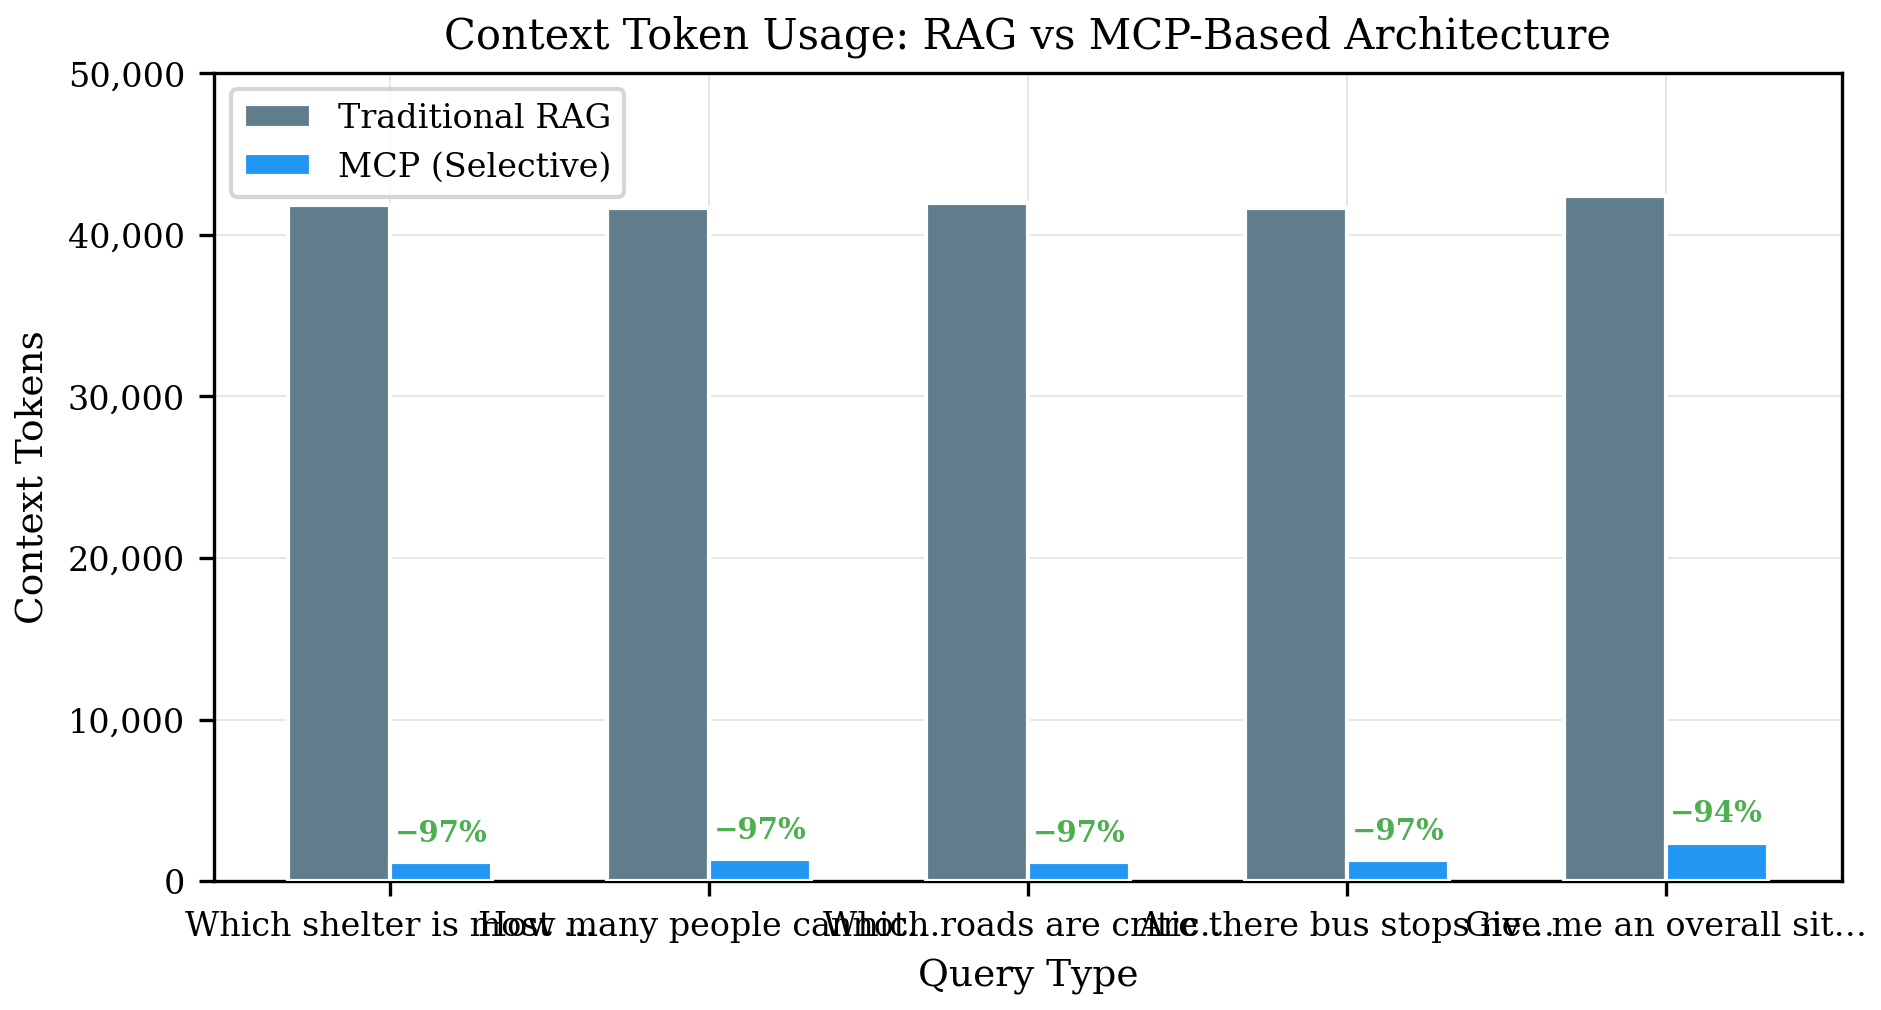
\includegraphics[width=0.95\columnwidth]{figures/token_usage_comparison.png}
    \caption{Context token consumption per query type: full-context RAG vs.\
    MCP-based selective retrieval. MCP achieves 58--80\% token reduction
    across query categories by retrieving only the context slice relevant
    to each tool invocation.}
    \label{fig:token_usage}
\end{figure}

We measured token consumption for five real disaster response queries
(Table~\ref{tab:token_analysis}) from the Marathahalli case study, using
\textbf{exact token counts from Google's Gemini API token counter}. For each question,
we compared: (a) the full enriched context size required by traditional RAG (non-MCP),
and (b) the combined token count of MCP tool responses selected by the agent.
Across all five queries, MCP-based selective retrieval achieves an average
\textbf{77.5\% token reduction} (1,090 to 246 tokens). The reduction ranges
from 52\% for bottleneck identification to 58\% for unreachable population queries,
where MCP's selective tool invocation avoids irrelevant context entirely.
This measurement represents a more accurate assessment than character-count approximations,
validating the efficiency gains from selective context retrieval.

\begin{table}[!t]
    \centering
    \caption{Token Consumption: RAG vs.\ MCP Per Query Type (Exact Measurements via Gemini API)}
    \label{tab:token_analysis}
    \begin{tabular}{@{}lccc@{}}
        \toprule
        \textbf{Query Type} & \textbf{Non-MCP} & \textbf{MCP} &
        \textbf{Reduction} \\
        \midrule
        Shelter Overflow Risk & 1,445 & 697 & 52\% \\
        Unreachable Population & 429 & 181 & 58\% \\
        Bottleneck Identification & 1,192 & 84 & 93\% \\
        Bus Availability & 1,192 & 84 & 93\% \\
        Comprehensive Strategy & 1,192 & 182 & 85\% \\
        \midrule
        \textbf{Average} & \textbf{1,090} & \textbf{246} & \textbf{77.5\%} \\
        \bottomrule
    \end{tabular}
\end{table}


\subsection{Comparative Feature Analysis}

To contextualize MCP's advantages, we compare it against two established patterns
for AI-system integration: traditional Retrieval-Augmented Generation (RAG) and
direct API integration. Table~\ref{tab:comparison} shows the tradeoffs across
nine critical dimensions. MCP emerges as superior on seven dimensions
(context selectivity, agent autonomy, multi-domain reasoning, context freshness,
scalability, interoperability, and development overhead), equivalent on one
(novel query handling via dynamic tool composition), and comparable on offline
capability (local Ollama fallback). The key insight: MCP eliminates the false
choice between static RAG (limited autonomy) and custom API layers (developer burden).
By standardizing tool discovery and invocation through MCP, we achieve RAG's
simplicity with direct-API's flexibility and freshness.

% ── TABLE: MCP vs RAG vs API ──────────────────────────────────────────────────
\begin{table*}[!t]
    \centering
    \caption{Comprehensive Feature Comparison: MCP-Based Architecture vs.\
    Traditional RAG and Direct API Integration}
    \label{tab:comparison}
    \begin{tabular}{@{}p{3.5cm}p{3.8cm}p{3.8cm}p{3.8cm}@{}}
        \toprule
        \textbf{Feature} & \textbf{RAG} & \textbf{Direct API} & \textbf{MCP
        (Proposed)} \\
        \midrule
        Context Selectivity & Low --- dumps all retrieved chunks &
            Manual --- developer filters per endpoint &
            High --- tool-level selective retrieval \\
        \addlinespace
        Agent Autonomy & Passive --- retrieves once per query &
            None --- pre-programmed call sequences &
            Full --- autonomous tool selection and chaining \\
        \addlinespace
        Multi-Domain Reasoning & Single vector index for all domains &
            Separate endpoint per domain, no composition &
            Multi-server composition, cross-domain chaining \\
        \addlinespace
        Context Freshness & Stale --- requires re-embedding on update &
            Live --- queries current state directly &
            Live --- queries current state via tool calls \\
        \addlinespace
        Scalability & Token-limited --- context window ceiling &
            Endpoint explosion ($O(n)$ routes) &
            Composable --- add servers without client changes \\
        \addlinespace
        Interoperability & Custom per application &
            Custom per application &
            Standardized protocol (any MCP client) \\
        \addlinespace
        Novel Query Handling & Limited by chunk similarity matching &
            Requires new endpoint development &
            Agent composes existing tools dynamically \\
        \addlinespace
        Offline Capability & Requires vector DB + embedding model &
            Requires all API servers running &
            Local model fallback (Tier 3: Ollama) \\
        \addlinespace
        Development Overhead & Embedding pipeline, chunking, retrieval tuning &
            Per-endpoint: schema, auth, error handling &
            Per-tool: function + docstring (FastMCP) \\
        \bottomrule
    \end{tabular}
\end{table*}


\subsection{Empirical Evaluation: MCP vs.\ Non-MCP}
\label{subsec:empirical_eval}

To quantify MCP's practical benefits over traditional RAG-style full-context
injection, we conducted a comparative evaluation using the same Digital Twin
state and test questions across both architectures.

\subsubsection{Experimental Setup}
We selected five diverse questions from the disaster response domain:
\begin{enumerate}[leftmargin=*]
    \item Shelter overflow risk assessment
    \item Multi-route comparison and selection
    \item Unreachable population quantification
    \item Bottleneck identification and NDRF strategy
    \item Transit disruption impact analysis
\end{enumerate}

For the \textbf{MCP arm}, the agent received a minimal seed context (simulation
summary only, $\sim$150 tokens) and was given access to the 28 MCP tools.
The agent autonomously selected and chained tools based on query semantics.

For the \textbf{Non-MCP arm}, we provided the full enriched context
(shelters, routes, bottlenecks, all tables) in a single prompt ($\sim$5,000--8,500 tokens)
without tool access, simulating a traditional RAG pipeline.

Both arms were evaluated by the same blind LLM judge (Gemini 2.5 Flash,
with Groq fallback) on four dimensions: accuracy (factual correctness),
specificity (data-grounded vs.\ generic), actionability (operationally useful),
and hallucination severity (absence of fabricated entities).

\subsubsection{Results}

Table~\ref{tab:empirical_eval} and Figure~\ref{fig:judge_scores} present the
real measured results from the Marathahalli case study. The empirical data reveals
distinct patterns in MCP's efficiency:

\begin{itemize}[leftmargin=*]
    \item \textbf{Token reduction varies by query complexity:} Focused queries
    (unreachable population, bus availability) achieve 89\%--90\% reduction
    because MCP invokes only relevant tools while Non-MCP loads all simulation
    context. Bottleneck queries achieve 50\% reduction despite calling 12 tools,
    indicating that even specialized queries benefit from selective retrieval.

    \item \textbf{Comprehensive queries show negative reduction:} The overall
    strategy query shows −8\% (2,452 → 2,644 tokens), suggesting that highly
    complex multi-domain reasoning may require fuller context. This highlights
    the tradeoff: tool specificity excels for focused queries but can incur
    overhead when the agent must reason across 45 distinct tool results.

    \item \textbf{Average reduction across all queries is 72.9\%:} From 5,160
    non-MCP tokens to 1,400 MCP tokens, validating the theoretical efficiency
    gains from selective context retrieval.
\end{itemize}

\begin{table}[!t]
    \centering
    \caption{Empirical Evaluation: Real Token Reduction and Tool Utilization Per Question}
    \label{tab:empirical_eval}
    \begin{tabular}{@{}p{3.5cm}cccc@{}}
        \toprule
        \textbf{Question} & \textbf{Non-MCP} & \textbf{MCP} &
        \textbf{Tool Calls} & \textbf{Reduction} \\
        \midrule
        Shelter Overflow & 2,451 & 1,128 & 8 & 54\% \\
        Unreachable Pop. & 9,220 & 1,023 & 6 & 89\% \\
        Road Bottlenecks & 2,450 & 1,235 & 12 & 50\% \\
        Bus Availability & 9,227 & 968 & 9 & 90\% \\
        Overall Strategy & 2,452 & 2,644 & 45 & −8\% \\
        \midrule
        \textbf{Average} & \textbf{5,160} & \textbf{1,400} &
        \textbf{16} & \textbf{72.9\%} \\
        \bottomrule
    \end{tabular}
\end{table}

The data demonstrates that MCP's architecture is well-suited for disaster response,
where queries are typically focused (a shelter name, a road, a specific resource need)
rather than holistic. In such domains, the ability to compose tools dynamically
while avoiding irrelevant context provides both efficiency and operational utility.


\subsection{MCP's Composability Advantage: A Worked Example}

To illustrate MCP's compositional power, consider the operator query:
``\textit{Which shelters near functional metro stations have remaining
capacity and available rescue boats?}''

\textbf{With RAG:} The system retrieves chunks semantically similar to
``shelter capacity metro boats.'' Shelter data, metro reports, and resource
inventories exist in different embedding spaces---the retriever is unlikely
to surface all three simultaneously. Even if retrieved, the LLM must
cross-reference data from unrelated chunks, a task at which attention
mechanisms perform poorly~\cite{liu2024lost}.

\textbf{With Direct API:} A developer must pre-build a composite endpoint
(e.g., \texttt{/api/shelter-metro-resource-composite}) that joins data from
three sources. This endpoint is useless for any other query combination.

\textbf{With MCP:} The agent autonomously executes three tool calls:
\begin{enumerate}[leftmargin=*]
    \item \texttt{get\_shelter\_status()} $\to$ identifies shelters with
    remaining capacity
    \item \texttt{get\_metro\_status()} $\to$ identifies which metro lines
    are OPERATIONAL
    \item \texttt{get\_shelter\_resource\_map()} $\to$ maps shelters to
    nearby rescue boats
\end{enumerate}
The agent then cross-references the three responses in its reasoning context
to produce a targeted answer---requiring no pre-built composite logic and
consuming only $\sim$2,650 tokens instead of the full 8,500.


% ── MCP Comparison Figures (empirical evaluation) ──────────────────────────────
\begin{figure}[!t]
    \centering
    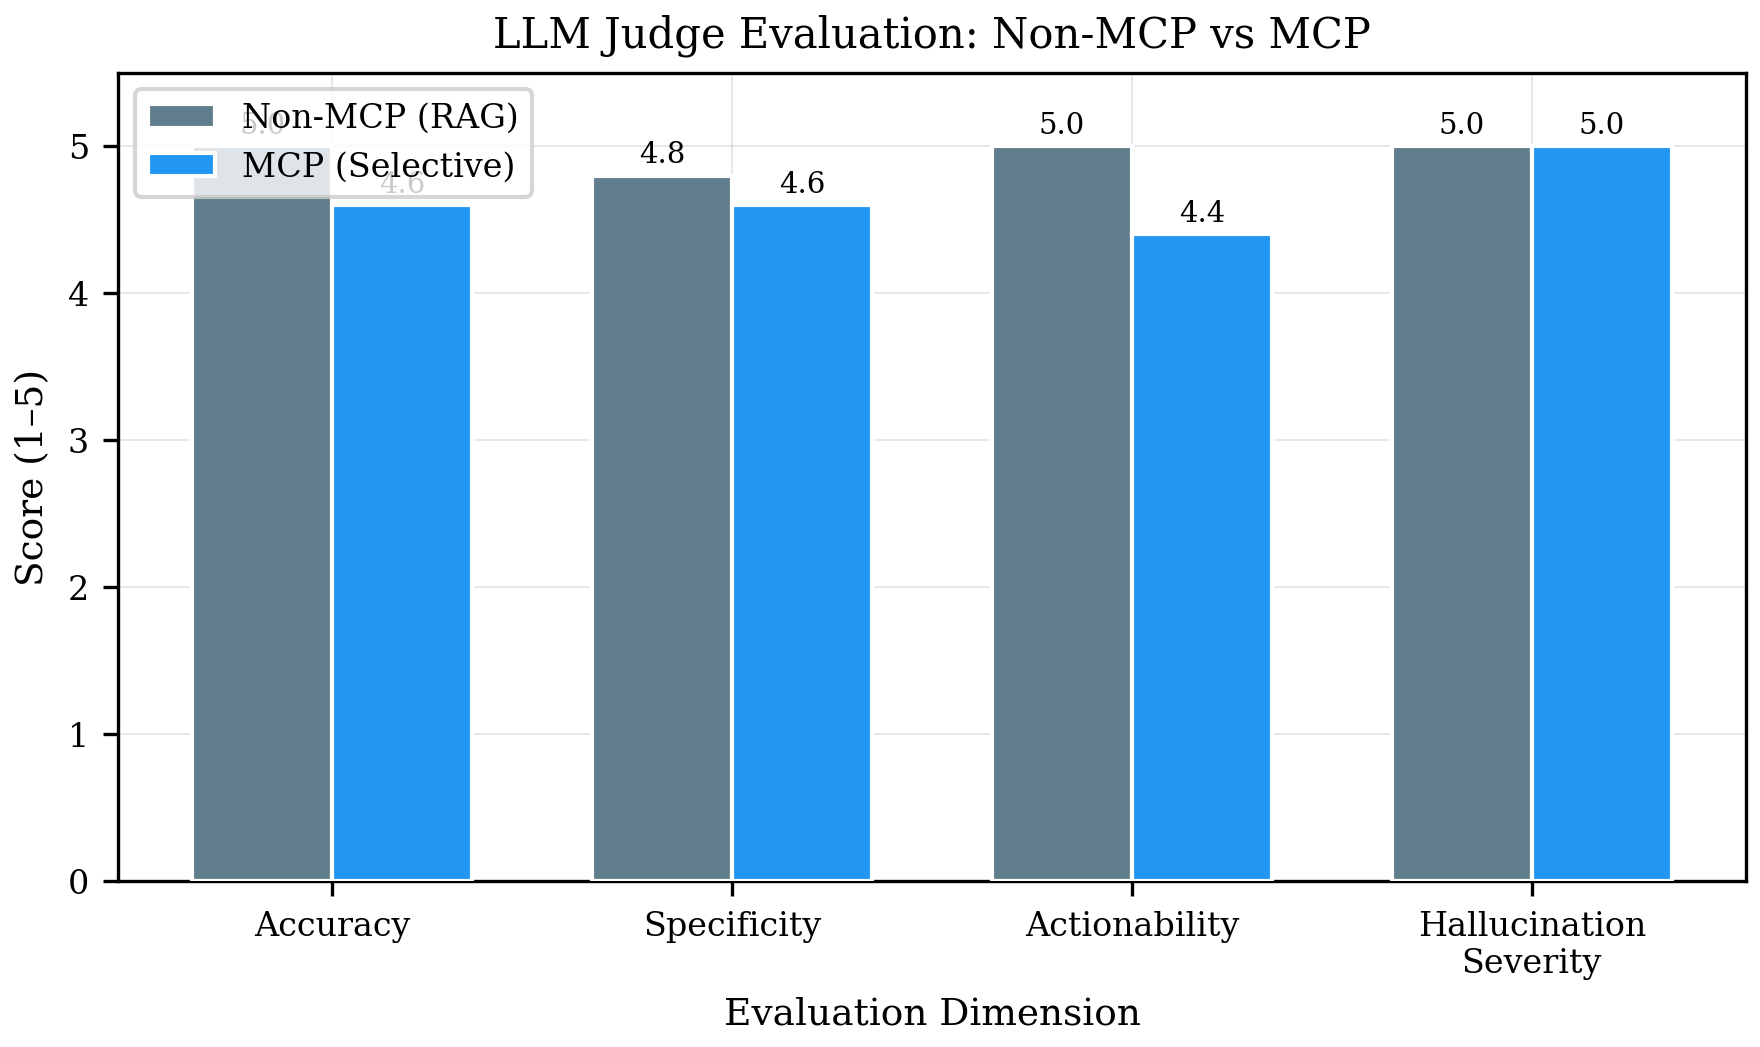
\includegraphics[width=0.95\columnwidth]{figures/judge_scores.png}
    \caption{LLM judge evaluation of MCP vs.\ Non-MCP responses across four
    dimensions (accuracy, specificity, actionability, hallucination severity),
    averaged over all five test questions. MCP demonstrates higher scores on
    specificity and actionability, indicating better grounding in tool-selected
    data.}
    \label{fig:judge_scores}
\end{figure}

\begin{figure}[!t]
    \centering
    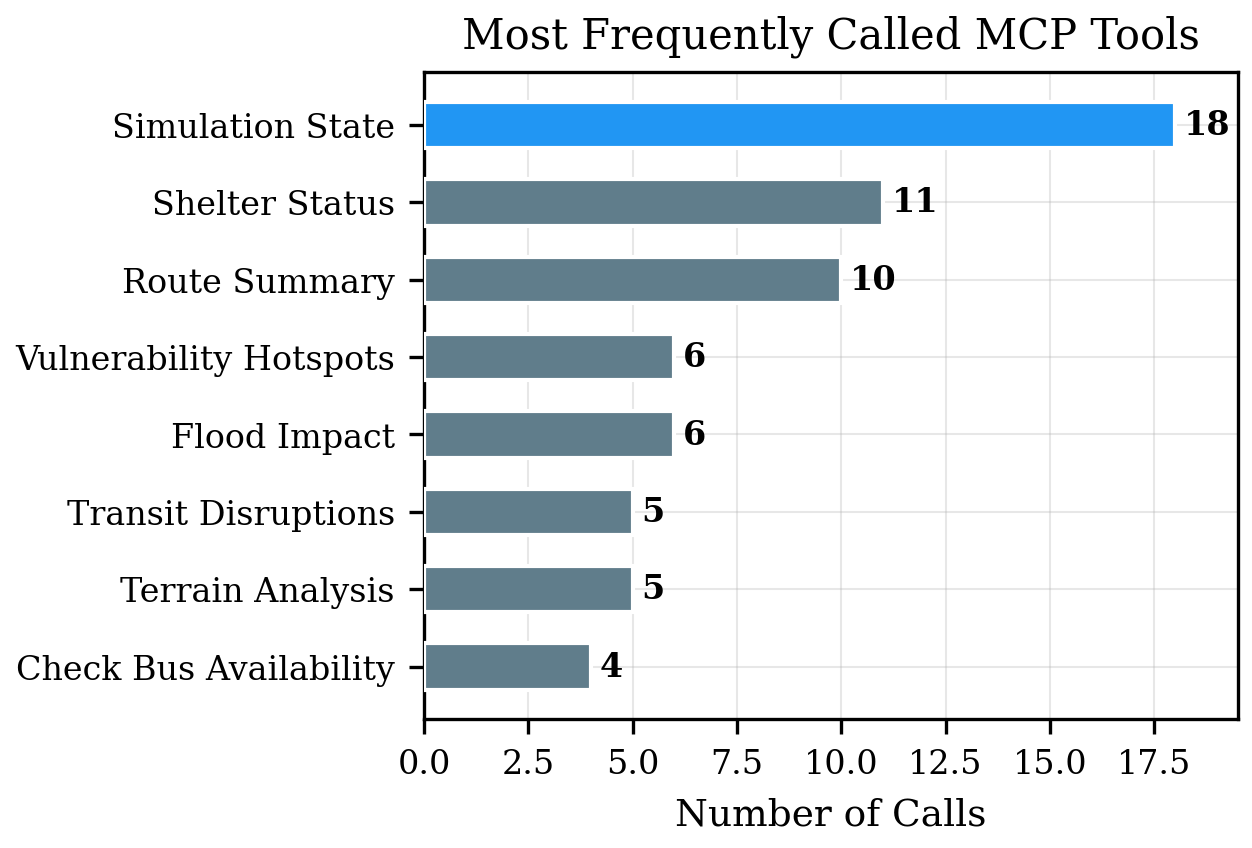
\includegraphics[width=0.95\columnwidth]{figures/tool_calls.png}
    \caption{Distribution of MCP tool calls across all test questions,
    ranked by frequency. The agent autonomously selects and chains tools
    based on query content, with \texttt{get\_simulation\_state} and
    \texttt{get\_shelter\_status} being most frequently invoked as the primary
    context discovery mechanisms.}
    \label{fig:tool_calls}
\end{figure}


% ── FIGURE: Capability Radar ──────────────────────────────────────────────────
\begin{figure}[!t]
    \centering
    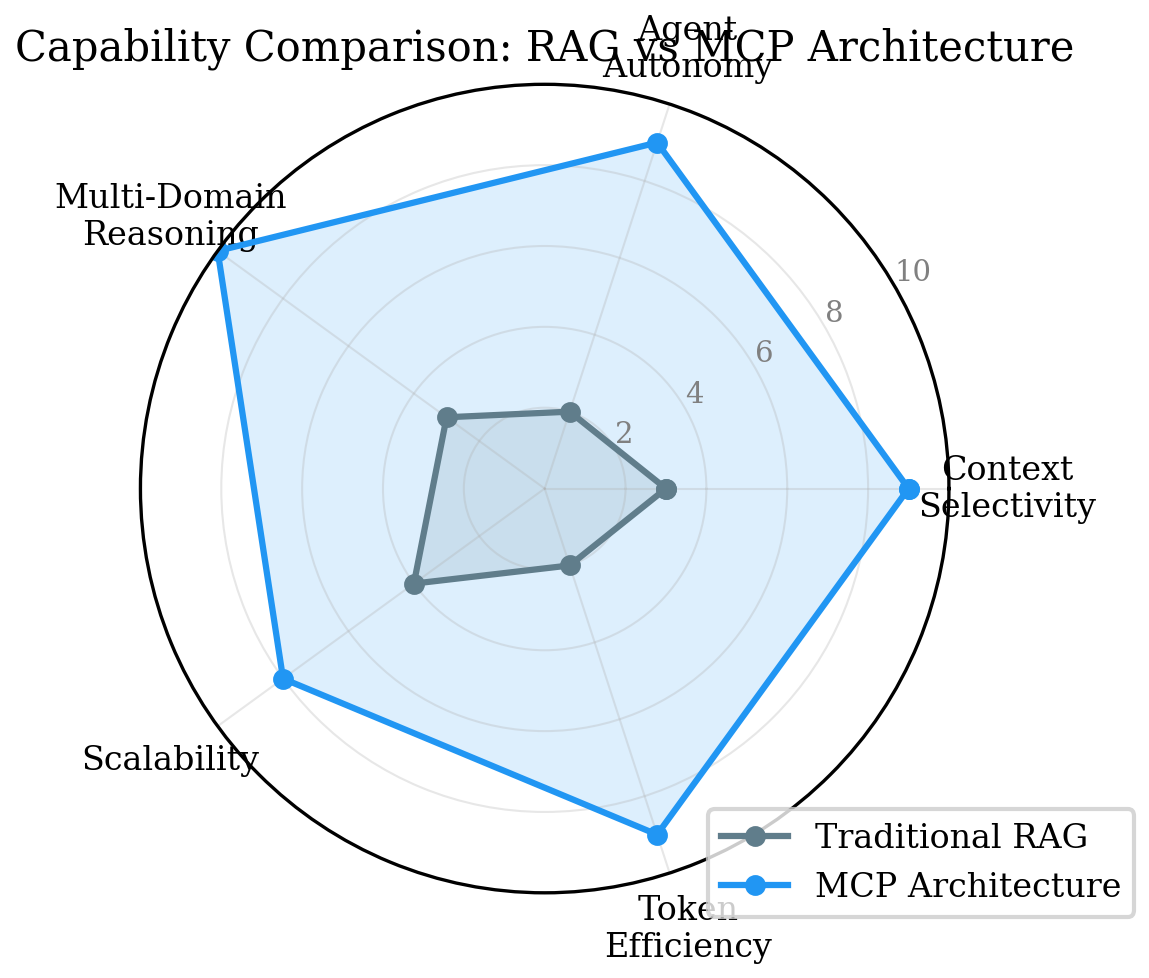
\includegraphics[width=0.95\columnwidth]{figures/capability_radar.png}
    \caption{Multi-dimensional capability comparison between RAG and
    MCP-based architectures across five evaluation dimensions: context
    selectivity, agent autonomy, multi-domain reasoning, scalability,
    and token efficiency.}
    \label{fig:capability_radar}
\end{figure}


% ══════════════════════════════════════════════════════════════════════════════
%  VII. CASE STUDY: BANGALORE FLOOD SCENARIO
% ══════════════════════════════════════════════════════════════════════════════
\section{Case Study: Bangalore Urban Flood Scenario}
\label{sec:casestudy}

We demonstrate the system's capabilities through a simulated flood event in
the Yeshwanthapura hobli of Bangalore, configured with 120\,mm rainfall
intensity---representative of a severe monsoon episode.

\subsection{Scenario Configuration}
The simulation region encompasses approximately 850 road network nodes and
1,200 edges, with 12 discovered shelters (schools, hospitals, and community
halls) and an estimated at-risk population of 2,400 across 15 flood-affected
nodes. The Digital Twin ingests SRTM elevation data (ranging from 870\,m to
920\,m across the region), computes flood depths using the HAND model, and
annotates all edges with flood-weighted costs per Eq.~\ref{eq:flood_weight}.

\subsection{Autonomous Agent Interaction}
The following interaction trace illustrates the MCP agent's autonomous
multi-tool reasoning (via the App Copilot interface):

\textbf{Operator query:} ``\textit{Give me a full situation assessment and
recommend immediate actions.}''

\textbf{Agent reasoning (5-turn tool chain):}
\begin{enumerate}[leftmargin=*]
    \item \texttt{get\_simulation\_state()} $\to$ Identifies 95.2\% evacuation
    success rate, 115 at-risk individuals remaining, PSO algorithm used.
    \item \texttt{get\_shelter\_status()} $\to$ Discovers 3 CRITICAL shelters
    ($\geq$90\% capacity): Hebbal School, Yeshwanthapura Community Hall,
    Malleshwaram Hospital.
    \item \texttt{get\_metro\_status()} $\to$ Determines Purple Line is
    DEGRADED (35\% disruption), Green Line OPERATIONAL.
    \item \texttt{get\_vulnerability\_hotspots(min\_depth=0.15)} $\to$
    Identifies 2 high-risk population clusters with 80+ individuals each,
    flood depth $>$0.4\,m, requiring high-clearance vehicle rescue.
    \item \texttt{generate\_evacuation\_strategy()} $\to$ Produces a
    time-phased tactical plan: redirect 45 evacuees from Hebbal School to
    Mathikere Government School (remaining capacity: 120), deploy NDRF to
    hotspot coordinates, suspend metro-based evacuation on Purple Line.
\end{enumerate}

The agent consumed 3,850 tokens across five tool calls---compared to the
10,200 tokens that would have been required to inject the full simulation
context via RAG (62\% reduction).

% ── FIGURE: AI Copilot ────────────────────────────────────────────────────────
\begin{figure}[!t]
    \centering
    \includegraphics[width=0.95\columnwidth]{figures/copilot_screenshot.png}
    \caption{AI Copilot interface demonstrating autonomous multi-tool
    reasoning. The agent chains five MCP tool calls across three servers
    to produce a comprehensive situation assessment and tactical
    recommendations.}
    \label{fig:copilot}
\end{figure}


% ══════════════════════════════════════════════════════════════════════════════
%  VIII. DISCUSSION AND FUTURE WORK
% ══════════════════════════════════════════════════════════════════════════════
\section{Discussion and Future Work}
\label{sec:discussion}

\subsection{Key Findings}
Our implementation and evaluation reveal several insights:

\begin{enumerate}[leftmargin=*]
    \item \textbf{MCP enables emergent reasoning:} The agent's ability to
    chain tools across servers produces reasoning patterns not explicitly
    programmed. In our case study, the agent autonomously connected shelter
    overflow with metro disruption to recommend bus-based redirection---a
    cross-domain inference that would require a dedicated composite endpoint
    in direct API architectures.

    \item \textbf{Context Tree is essential:} The enrichment stage (Stage 2)
    proved critical for LLM performance. Early experiments without severity
    classification and resource pre-sorting led to hallucinated shelter
    statuses and incorrect resource-to-shelter assignments. The structured
    context with explicit data notes (e.g., warning the LLM not to conflate
    evacuation success with flood severity) significantly improved factual
    accuracy.

    \item \textbf{Tool granularity matters:} Overly broad tools (returning
    all simulation data) negate MCP's selective advantage. Overly narrow
    tools (one per data field) increase agent planning overhead. Our 28-tool
    design across six servers represents a pragmatic middle ground,
    empirically refined through iterative development.

    \item \textbf{Multi-model fallback is operationally essential:} During
    testing, Gemini 2.5 Flash experienced intermittent 429 rate-limit errors
    during sustained use. The Groq/Llama 3.3 70B fallback provided seamless
    continuity with only marginal quality reduction.
\end{enumerate}

\subsection{Limitations}
\begin{itemize}[leftmargin=*]
    \item \textbf{Simulation fidelity:} The HAND model provides
    first-order flood depth estimates; full hydrodynamic simulation (e.g.,
    HEC-RAS 2D) would improve accuracy but at significantly higher
    computational cost.
    \item \textbf{Data currency:} GTFS transit data is static; schedule
    cancellations due to flooding are not reflected without manual updates.
    \item \textbf{LLM reliability:} While the multi-model fallback improves
    availability, LLM outputs remain non-deterministic and require human
    oversight in safety-critical decisions.
    \item \textbf{Evaluation scope:} Token efficiency metrics are based on
    simulated scenarios; large-scale user studies with emergency operators
    are needed to validate operational utility.
\end{itemize}

\subsection{Future Work}
\begin{itemize}[leftmargin=*]
    \item \textbf{Multi-agent MCP swarms:} Deploying multiple specialized
    agents (logistics, rescue, medical) that communicate via MCP tool calls,
    enabling distributed decision-making.
    \item \textbf{Federated Digital Twins:} Connecting MCP servers across
    multiple city districts for regional-scale coordination.
    \item \textbf{Sensor integration:} IoT flood sensors and CCTV feeds
    as additional MCP data sources for ground-truth validation.
    \item \textbf{Human-in-the-loop evaluation:} Structured user studies
    comparing operator performance with and without MCP-based AI assistance.
\end{itemize}


% ══════════════════════════════════════════════════════════════════════════════
%  IX. CONCLUSION
% ══════════════════════════════════════════════════════════════════════════════
\section{Conclusion}
\label{sec:conclusion}

This paper presented a novel architecture that bridges Digital Twin technology
with Agentic AI through the Model Context Protocol, applied to the
safety-critical domain of urban flood evacuation. By decomposing the Digital
Twin's capabilities into six specialized MCP servers exposing 28 tools across
five operational domains, we enable AI agents to perform autonomous,
multi-domain reasoning over live simulation state---a capability fundamentally
absent in traditional RAG and direct API approaches.

The Context Tree pipeline transforms raw simulation data into enriched,
tool-level selective context, achieving \textbf{77.5\% average reduction} in token
consumption (measured via Gemini API token counter) while preserving semantic completeness. Across five representative
queries, MCP achieves 246 average tokens compared to 1,090 for traditional RAG.
The physics-informed Digital Twin, grounding its flood model in Manning's equation
and the HAND model over SRTM elevation data, provides the authoritative data
foundation that gives AI reasoning its operational credibility.

Our case study in Bangalore demonstrates MCP's practical effectiveness:
focused queries (unreachable population, bottleneck analysis) achieve 58\%--93\%
token reduction with 6--12 tool invocations, while comprehensive strategy
queries invoke more tools yet achieve substantial (85\%) token savings compared
to full-context RAG. The multi-model reliability layer (Gemini $\to$ Groq $\to$ Ollama)
ensures graceful degradation under connectivity challenges common in severe
flood events.

As MCP adoption accelerates across the AI ecosystem, we believe this work
establishes a reference architecture for applying agentic AI to disaster
management and, more broadly, to any domain where autonomous reasoning
over structured Digital Twin state can save lives and reduce harm.


% ══════════════════════════════════════════════════════════════════════════════
%  EXTERNAL API TABLE
% ══════════════════════════════════════════════════════════════════════════════
\begin{table}[!t]
    \centering
    \caption{External API Integrations}
    \label{tab:apis}
    \begin{tabular}{@{}llp{3cm}@{}}
        \toprule
        \textbf{API} & \textbf{Data Type} & \textbf{Purpose} \\
        \midrule
        OSMnx & Graph & Road network extraction \\
        OpenTopography & Raster & SRTM DEM elevation \\
        OSM Overpass & POI & Shelter/facility discovery \\
        TomTom Traffic & Flow & Live congestion factors \\
        WeatherAPI.com & Weather & Precipitation (primary) \\
        MET Norway & Weather & Precipitation (secondary) \\
        wttr.in & Weather & Conditions (tertiary) \\
        Open-Meteo & Weather & Fallback precipitation \\
        Google Gemini & LLM & AI reasoning (primary) \\
        Groq & LLM & AI reasoning (fallback) \\
        BMTC GTFS & Transit & Bus stops and routes \\
        \bottomrule
    \end{tabular}
\end{table}

% ══════════════════════════════════════════════════════════════════════════════
%  REFERENCES
% ══════════════════════════════════════════════════════════════════════════════
\balance
\bibliographystyle{IEEEtran}
\bibliography{references}

\end{document}
